\documentclass[a4paper,12pt,french]{article}

\usepackage[cours]{../../../Style}

\renewcommand\tabularxcolumn[1]{m{#1}}

% Début du document
%%%%%%%%%%%%%%%%%%%
\begin{document}

\title{Suites: Généralités}
\author{}
\date{}
\maketitle

%\begin{FlushLeft}

\section{Premières définitions}

\begin{defin}
Une suite est une séquence ordonnée de nombres réels.
\end{defin}

\begin{exs}
La suite des nombres pairs est $0;2;4; \ldots$
\end{exs}

\begin{defin}
Une suite peut être vue comme une fonction $\fonction u {\N} {\R} n {u(n)}$. On notera plutôt $u_n$ ($u$ indice $n$) au lieu de $u(n)$.
\end{defin}

\begin{rmq}
Par défaut, on numérote une suite à partir de $0$, mais on peut aussi commencer à n'importe quel entier.
\end{rmq}

\begin{exs} \saut
\begin{itemize}
\item Reprenons la suite $u$ des nombres pairs. Le premier nombre pair est $0$, on peut alors noter $u_0=0$, puis $u_1=2, \ldots$ On pourrait aussi commencer la numérotation à partir de $1$. On aurait alors $u_1=0, u_2=2, \ldots$. $u_0$ ne serait alors pas défini.
\item On prend la suite $u$ de nombres suivants: $0,\ 1,\ 3,\ 6,\ 10,\ \ldots$. Si son premier terme ( $0$ ) est d'indice 23, alors son quatrième terme ( $6$ ) est le terme d'indice 26.
\end{itemize}
\end{exs}
 
\rem{Exos 12->15 et 21->24 p90} 
 
\section{Modes de générations de suites}

\begin{fait}[defin]
Une suite peut être générée de trois manières différentes:
\end{fait}

\subsection{Par une expression explicite}

\begin{defin}
Il s'agit d'une suite vérifiant $u_n=f(n)$ avec $f$ une fonction.
\end{defin}

\begin{ex}
On se donne la suite $(u_n)$ définie pour tout entier naturel $n$ par $u_n=n^2-3n$.

\begin{center}
\begin{tabularx}{0.7\linewidth}{ 
  | >{\centering\arraybackslash}c 
  | >{\centering\arraybackslash}X
  | >{\centering\arraybackslash}X
  | >{\centering\arraybackslash}X
  | >{\centering\arraybackslash}X
  | >{\centering\arraybackslash}X
  | >{\centering\arraybackslash}X
  | >{\centering\arraybackslash}X| } \hline
$n$ & 0 & 1 & 2 & 3 & 4 & 5 & 6\\ \hline
$u_n$ & 0 & $-2$ & $-2$ & $0$ & $4$ & $10$ & $18$ \\ \hline %\rule[-7pt]{0pt}{30pt}
\end{tabularx}
\end{center}

\end{ex}

\subsection{Par une relation de récurrence}

\begin{defin}
Définir une suite par récurrence revient à donner son premier terme puis une relation permettant de calculer le terme suivant à partir du précédent.
\end{defin}

\begin{exs} \saut
\begin{itemize}
\item On se donne la suite $(v_n)$ dont le premier terme est $1$ et dont le terme suivant est obtenu en doublant le terme précédent. On a alors $v_0= 1$, $v_1$ est le double de $v_0$ donc $v_1=2 \times v_0=2$, puis de même $v_3=4,\ v_4=8,\ v_5=16 \ldots$ Pour résumer cette relation, on note $u_{n+1} = 2 \times u_n$.
\end{itemize}
\begin{center}
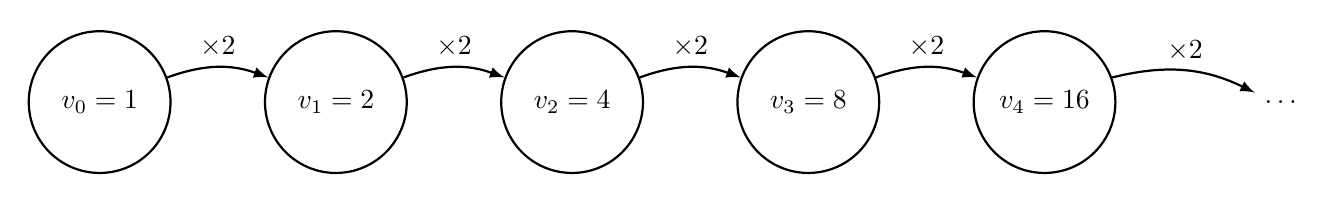
\begin{tikzpicture}[scale=1]
\node[draw,circle,thick, minimum size=18mm] (W0) at (-3,0) {$v_0=1$};
\node[draw,circle,thick, minimum size=18mm] (W1) at (0,0) {$v_1=2$};
\node[draw,circle,thick, minimum size=18mm] (W2) at (3,0) {$v_2=4$};
\node[draw,circle,thick, minimum size=18mm] (W3) at (6,0) {$v_3=8$};
\node[draw,circle,thick, minimum size=18mm] (W4) at (9,0) {$v_4=16$};
\node (W5) at (12,0) {$\ldots$};
\draw[->,>=latex,thick] (W0) to[bend left=20] node[midway,above]{$\times 2$} (W1);
\draw[->,>=latex,thick] (W1) to[bend left=20] node[midway,above]{$\times 2$} (W2);
\draw[->,>=latex,thick] (W2) to[bend left=20] node[midway,above]{$\times 2$} (W3);
\draw[->,>=latex,thick] (W3) to[bend left=20] node[midway,above]{$\times 2$} (W4);
\draw[->,>=latex,thick] (W4) to[bend left=20] node[midway,above]{$\times 2$} (W5);
\end{tikzpicture}
\end{center}

\begin{itemize}
\item Soit $(w_n)$ la suite définie par $w_0=0$ et pour tout entier naturel $n$, $w_{n+1}=2w_n+1$. Alors $w_1=2w_0+1=2 \times 0 + 1=1 \ , \ w_2=2w_1+1=3 \ , \ w_3=7 \ldots$
\end{itemize}
\begin{center}
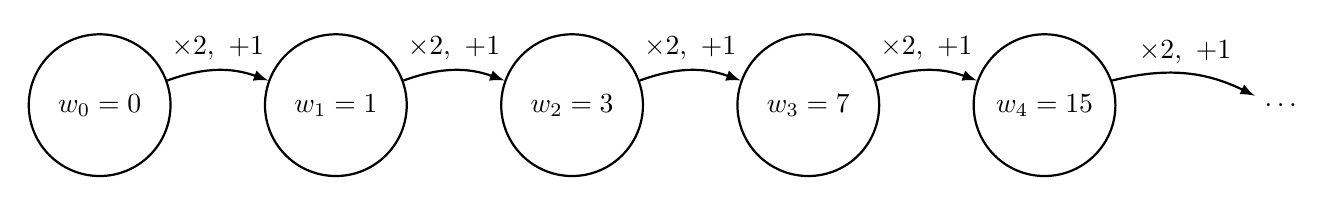
\begin{tikzpicture}[scale=1]
\node[draw,circle,thick, minimum size=18mm] (W0) at (-3,0) {$w_0=0$};
\node[draw,circle,thick, minimum size=18mm] (W1) at (0,0) {$w_1=1$};
\node[draw,circle,thick, minimum size=18mm] (W2) at (3,0) {$w_2=3$};
\node[draw,circle,thick, minimum size=18mm] (W3) at (6,0) {$w_3=7$};
\node[draw,circle,thick, minimum size=18mm] (W4) at (9,0) {$w_4=15$};
\node (W5) at (12,0) {$\ldots$};\draw[->,>=latex,thick] (W0) to[bend left=20] node[midway,above]{$\times 2,\ + 1$} (W1);
\draw[->,>=latex,thick] (W1) to[bend left=20] node[midway,above]{$\times 2,\ + 1$} (W2);
\draw[->,>=latex,thick] (W2) to[bend left=20] node[midway,above]{$\times 2,\ + 1$} (W3);
\draw[->,>=latex,thick] (W3) to[bend left=20] node[midway,above]{$\times 2,\ + 1$} (W4);
\draw[->,>=latex,thick] (W4) to[bend left=20] node[midway,above]{$\times 2,\ + 1$} (W5);
\end{tikzpicture}
\end{center}

\end{exs}

\subsection{Par une définition plus abstraite}

\begin{ex}
Soit $(w_n)$ la suite des chiffres de l'écriture décimale de $\sqrt 2 = 1.414213\ldots$. Alors $w_0=1 \ , \ w_1=4 \ , \ w_2=1 \ , \ w_3=4 \ , \ w_4=2 \ , \ \ldots$
\end{ex}

\subsection{Un exemple pour résumer}

\begin{ex}
On se donne les trois suites suivantes:
\begin{itemize}
\item La suite $u$ des nombres pairs.
\item La suite $v$, qui vérifie pour tout $n \in \N, u_n=2n$.
\item La suite $w$ telle que $w_0=0$, et pour tout $n \in \N, w_{n+1}=w_n+2$.
\end{itemize}

\begin{center}
\begin{tabularx}{0.7\linewidth}{ 
  | >{\centering\arraybackslash}c 
  | >{\centering\arraybackslash}X
  | >{\centering\arraybackslash}X
  | >{\centering\arraybackslash}X
  | >{\centering\arraybackslash}X
  | >{\centering\arraybackslash}X
  | >{\centering\arraybackslash}X
  | >{\centering\arraybackslash}X| } \hline
$n$ & 0 & 1 & 2 & 3 & 4 & 5 & 6\\ \hline
$u_n$ & 0 & 2 & 4 & 6 & 8 & 10 & 12 \\ \hline %\rule[-7pt]{0pt}{30pt}
$v_n$ & 0 & 2 & 4 & 6 & 8 & 10 & 12 \\ \hline
$w_n$ & 0 & 2 & 4 & 6 & 8 & 10 & 12 \\
\hline
\end{tabularx}
\end{center}

En fait, on peut montrer que ces trois suites sont égales.
\end{ex}

\rem{
On peut définir des suites plus compliquées par récurrence, par exemple à partir de deux termes initiaux: $u_0=2,u_1=3$ et $u_{n+2}=u_{n+1}-2u_n$ \\
C'est la définition par récurrence qui donne du sens aux suites, mais elle peut être plus difficile à manipuler. Dans la pratique, la définition par une fonction est préférable. Il existe des méthodes plus ou moins poussées pour passer d'une notation à une autre (hors programmes). \\
Exos 20,25,26,43,45,46,48,(54) \\
Pour ceux qui ont de l'avance: 28,47,50,51
}

\section{Représentation graphique d'une suite}
\begin{methode}
On peut représenter une suite $(u_n)$ dans un repère du plan en plaçant les points $(n,u_n)$ pour $n \in \N$.
\end{methode}

\begin{ex}
En prenant la suite $(v_n)$ définie par $\left\{ \begin{aligned} &v_0=0 \\ &v_{n+1}=v_n^2-1 \end{aligned} \right.$, on obtient:
\begin{center}
\begin{tikzpicture}[scale=\echellepgf]
\begin{axis}[
styleglobal,
width=0.8*\echellepgfinv*\linewidth,
xmin=0, xmax=5,
ymin=-1.5, ymax=1,
xtick distance=0.5,
ytick distance=0.5
]
\addplot[samples=7,ultra thick,domain=(0:6),only marks]{0.5*(-1)^x-0.5};
\node[above right] at (0,0) {$(0;u_0)$};
\node[above right] at (4,0) {$(4;u_4)$};
\end{axis}
\end{tikzpicture}
\end{center}
\end{ex}

\rem{Calculer des valeurs à la main avant de faire le graphique\\Exos 17,18,19, si besoin: 58,60}

\section{Sens de variation d'une suite}

\begin{defin} Soit $u=(u_n)$ une suite.
\begin{itemize}
\item On dit que la suite $u$ est \textbf{croissante} lorsque pour tout $n \in \N, u_{n+1} \geq u_n$, autrement dit lorsque $u_{n+1}-u_n \geq 0$.
\item $u$ est dite \textbf{décroissante} lorsque pour tout $n \in \N, u_{n+1} \leq u_n$, autrement dit lorsque $u_{n+1}-u_n \leq 0$.
\item $u$ est dite \textbf{constante} lorsque pour tout $n \in \N, u_{n+1} = u_n$, autrement dit lorsque $u_{n+1}-u_n = 0$.
\end{itemize}
\end{defin}

\begin{ex}
On se donne la suite $(u_n)$ définie pour tout $n \in \N$ par $u_n=3-n$. On a $u_{n+1}-u_n=3-(n+1)-\left( 3-n\right)=\cancel 3 \cancel{-n}-1 \cancel{-3}+\cancel n=-1 \leq 0$ donc la suite $u$ est décroissante.
\end{ex}

\rem{Exos 31,59,61,65->68}

\begin{deroule}
\item \textbf{Total: 3.5 semaines}
\item Semaine 1
\begin{itemize} 
\item 30m - Activité intro ( promenade )
\item 30m - Début du cours: I
\item 1h30 - Exercices livre : Def suites
\item 30m - Activité récurrence
\end{itemize}
\item Vacances - Semaine 2  
\begin{itemize}
\item 20m - Cours II à compléter
\item 2h - Exercices livre
\item 1h30 - Cours III et Exos
\end{itemize}
\item Semaine 3
\begin{itemize}
\item 2h - Cours IV et exos
\end{itemize}
\end{deroule}
\begin{comment}

\rem{Modes de génération a détailler, un par un avec exs, Grande partie dessus, plusieurs exemples, rec a bien détailler, en faire plus, commencer par les exs a loral}

\rem{Activité pas modéliser, détailler a fond, donner les suites, aider tableur}

\rem{Définitions partout pour le II ? On perd peut-être un côté organique}

\section{Modes de générations de suites}

Une suite peut être générée de trois manières différentes:

\subsection{Par une expression explicite}

Il s'agit d'une suite vérifiant $u_n=f(n)$ avec $f$ une fonction.

\begin{ex}
On se donne la suite $(u_n)$ définie pour tout entier naturel $n$ par $u_n=n^2-3n$. Alors $u_0=0 \ , \ u_1=-2 \ , \ u_2=-2 \ , \ u_3=0 \ , \ u_4=4 \ldots$
\end{ex}

\subsection{Par une relation de récurrence}

On donne le premier terme $u_0$ de la suite puis une relation permettant de calculer le terme suivant à partir du précédent.

\begin{exs} \
\begin{itemize}
\item On se donne la suite $(v_n)$ dont le premier terme est $1$ et dont le terme suivant est obtenu en doublant le terme précédent. On a alors $v_0= 1$, $v_1$ est le double de $v_0$ donc $v_1=2 \times v_0=2$, puis de même $v_3=4,\ v_4=8,\ v_5=16 \ldots$ Pour résumer cette relation, on note $u_{n+1} = 2 \times u_n$.

\item Soit $(w_n)$ la suite définie par $w_0=0$ et pour tout entier naturel $n$, $w_{n+1}=2w_n+1$. Alors $w_1=2w_0+1=2 \times 0 + 1=1 \ , \ w_2=2w_1+1=3 \ , \ w_3=7 \ldots$
\end{itemize}

\begin{center}
\resizebox{\linewidth}{!}{
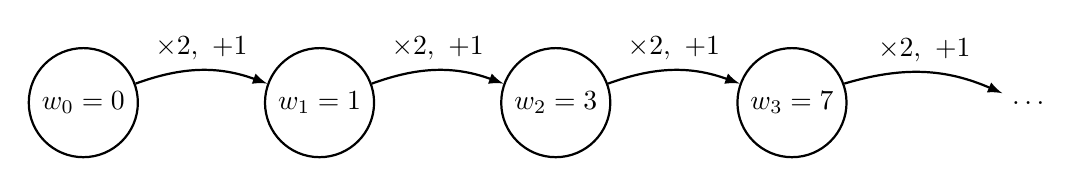
\begin{tikzpicture}[scale=1]
\node[draw,circle,thick] (W0) at (-3,0) {$w_0=0$};
\node[draw,circle,thick] (W1) at (0,0) {$w_1=1$};
\node[draw,circle,thick] (W2) at (3,0) {$w_2=3$};
\node[draw,circle,thick] (W3) at (6,0) {$w_3=7$};
\node (W4) at (9,0) {$\ldots$};\draw[->,>=latex,thick] (W0) to[bend left=20] node[midway,above]{$\times 2,\ + 1$} (W1);
\draw[->,>=latex,thick] (W1) to[bend left=20] node[midway,above]{$\times 2,\ + 1$} (W2);
\draw[->,>=latex,thick] (W2) to[bend left=20] node[midway,above]{$\times 2,\ + 1$} (W3);
\draw[->,>=latex,thick] (W3) to[bend left=20] node[midway,above]{$\times 2,\ + 1$} (W4);
\end{tikzpicture}}
\end{center}

\end{exs}

\subsection{Par une définition plus abstraite}

\begin{ex}
Soit $(w_n)$ la suite des décimales de $\sqrt 2 = 1.414213\ldots$. Alors $w_0=4 \ , \ w_1=1 \ , \ w_2=4 \ , \ w_3=2 \ldots$
\end{ex}

\subsection{Pour résumer}

On se donne la suite $u$ des nombres pairs. Cette définition est abstraite. On pourra vérifier que les définitions suivantes génèrent la même suite:
\begin{itemize}
\item Pour tout $n \in \N, u_n=2n$
\item $u_0=0$ et pour tout $n \in \N, u_{n+1}=u_n+2$.
\end{itemize}

\end{comment}

\end{document}
